% -*- latex -*-

This chapter documents the implementation and API of the Dax toolkit. This
documentation is primarily in reference to users of the Dax toolkit but
also gives some details on the internal implementation.

The Dax toolkit is written in C++ and makes extensive use of templates. The
toolkit is implemented as a header library, meaning that all the code is
implemented in header files (with extension \textfilename{.h}) and
completely included in any code that uses it. This is typically necessary
of template libraries, which need to be compiled with template parameters
that are not known until they are used. This also provides the convienience
of allowing the compiler to inline user code for better performance.

When documenting the Dax API, the following conventions are used.
\begin{itemize}
\item Filenames are printed in a \textfilename{sans serif font}.
\item C++ code is printed in a \textcode{monospace font}.
\item Macros and namespaces from the Dax toolkit are printed
  in \textnamespace{red}.
\item Identifiers from the Dax toolkit are printed in
  \textidentifier{blue}.
\item Signatures, described in Section~\ref{sec:GenericScheduling}, are
  printed in \textsignature{green}.
\end{itemize}

\section{Package Structure}
\label{sec:PackageStructure}

\index{packages|seealso{namespace}}
\index{packages|(}

The Dax toolkit is organized in a hierarchy of nested packages. The Dax
toolkit places definitions in \keyterm{namespaces} \index{namespace} that
correspond to the package (with the exception that one package may
specialized a template defined in a different namespace). Hence, the
description and

The base package is named \dax{}. All classes within the Dax toolkit are
placed either directly in the \dax{} package or in a package beneath
it. This helps prevent name collisions between the Dax toolkit and any
other library.

As described in Section~\ref{sec:StructureOfDaxFramework}, the Dax API is
divided into two distinct environments: \index{environments} the control
environment \index{control~environment} and the execution
environment. \index{execution~environment} The API for these two
environments are located in the \daxcont{} and \daxexec{} packages,
respectively. Items located in the base \dax{} namespace are available in
both environments.

Although it is conventional to spell out names in identifiers (see the
coding conventions in Section~\ref{sec:CodingConventions}), there is an
exception to abbreviate control and execution to \textnamespace{cont}
and \textnamespace{exec}, respectively. This is because it is also part of
the coding convention to declare the entire namespace when using an
identifier that is part of the corresponding package. The shorter names
make the identifiers easier to read, faster to type, and more feasible to
pack lines in 80 column displays. These abbreviations are also used instead
of more common abbreviations (e.g. ctrl for control) because, as part of
actual English words, they are easier to type.

Worklets provided by the Dax toolkit, described in
Section~\ref{sec:ProvidedWorklets}, are contained in the \daxworklet{}
package. Although the operation of a worklet happens exclusively in the
execution environment, worklets are typically initialized in the control
environment. Thus, the \daxworklet{} package is not encapsulated in either
\daxcont{} or \daxexec{}.

The Dax toolkit provides a base set of library functions that are ported to
the various systems and compilers on which it is used. These functions are
located in the \daxmath{} package. The features in \daxmath{} are available
in both the control and execution environments, but they are typically used
in the execution environment.

The Dax toolkit contains code that uses specalized compiler features, such
as those with CUDA and OpenMP, or libraries, such as Intel Threading
Building Blocks, that will not be available on all machines. Code for these
features are encapsulated in their own packages: \daxcuda{}, \daxopenmp{},
and \daxtbb{}. Within each one of these packages, there will
be \textnamespace{cont} and \textnamespace{exec} namespaces as necessary to
denote features that are accessible in only one environment or the other.

The Dax toolkit contains OpenGL interoperability \index{OpenGL}
\index{interoperability} that allows data generated with Dax to be
efficiently transfered to OpenGL objects. This feature is encapsulated in
the \daxopengl{} package.

Figure~\ref{fig:Packages} provides a diagram of the Dax package hierarchy.

\begin{figure}
  \centering
  %% \begin{itemizetight}
  %% \item \textnamespace{dax}
  %%   \begin{itemizetight}
  %%   \item \textnamespace{cont}
  %%   \item \textnamespace{exec}
  %%   \item \textnamespace{worklet}
  %%   \item \textnamespace{math}
  %%   \item \textnamespace{cuda}
  %%     \begin{itemizetight}
  %%     \item \textnamespace{cont}
  %%     \end{itemizetight}
  %%   \item \textnamespace{openmp}
  %%     \begin{itemizetight}
  %%     \item \textnamespace{cont}
  %%     \end{itemizetight}
  %%   \item \textnamespace{tbb}
  %%     \begin{itemizetight}
  %%     \item \textnamespace{cont}
  %%     \end{itemizetight}
  %%   \item \textnamespace{opengl}
  %%   \end{itemizetight}
  %% \end{itemizetight}
  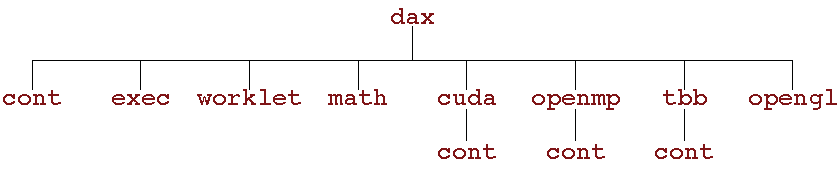
\includegraphics{images/PackageHierarchy}
  \caption{Dax package hierarchy.}
  \label{fig:Packages}
\end{figure}

By convention all classes will be defined in a file with the same name as
the class name (with a \textfilename{.h} extension) located in a directory
corresponding to the package name. For example, the \daxcont{ArrayHandle}
class is found in the \daxheader{dax/cont}{ArrayHandle.h} header. There
are, however, exceptions to this rule. Some smaller classes and types are
grouped together for convienience. These exceptions will be noted as
necessary.

Within each namespace there may also
be \textnamespace{internal}\indexnamespaceone{internal}
and \textnamespace{detail}\indexnamespaceone{detail}
sub-namespaces. The \textnamespace{internal} namespaces contain features
that are used internally and may change without
notice. The \textnamespace{detail} namespaces contain features that are
used by a particular class but must be declared outside of that
class. Users should generally ignore classes in these namespaces.

\index{packages|)}


\section{Basic Provisions}
\label{sec:BasicProvisions}

This section describes the core facilities provided by the Dax
toolkit. These include macros, types, and classes that define the
environment in which code is run, the core types of data stored, and
template introspection.

\subsection{Function and Method Exports}
\label{sec:FunctionAndMethodExports}

Any function or method defined by the Dax toolkit must come with an export
modifier that determines in which environments the function may be
run. These export modifiers are C macros that Dax uses to instruct the
compiler for which architectures to compile each method. Most user code
outside of the Dax toolkit need not use these macros with the important
exception of any classes passed to the Dax toolkit. This occurs when
defining new worklets, array containers, and device adapters.

Dax provides three export macros, \daxcontexport, \daxexecexport, and
\daxexeccontexport, which are used to declare functions and methods that
can run in the control environment, export environment, and both
environments, respectively. These macros get defined by including just
about any Dax header file, but including \daxheader{dax}{Types.h} will
ensure they are defined. 

The export macro is place after the template declaration, if there is one,
and before the return type for the function. Here is a simple example of a
function that will square a value. Since most types you would use this
function on have operators in both the control and execution environments,
the function is exported to both places.

\begin{daxexample}{Usage of export macro.}
template<class ValueType>
DAX_EXEC_CONT_EXPORT
ValueType Square(const ValueType &inValue)
{
 return inValue * inValue;
}
\end{daxexample}

The primary function of the export macros is to interject compiler-specific
keywords that specify what architecture to compile code for. For example,
when compiling with CUDA\index{CUDA}, the control exports have
\textcode{\_\_host\_\_} in them and execution exports have
\textcode{\_\_device\_\_} in them.

There is one additional export macro that is not used for functions but
rather used when declaring a constant data object that is used in the
execution environment. This macro is named
\daxmacro{DAX\_EXEC\_CONSTANT\_EXPORT}\index{export!constant}\index{constant~export}
and is used to declare a constant lookup table used when executing a
worklet. Its primary reason for existing is to add a
\textcode{\_\_constant\_\_} keyword when compiling with CUDA. This export
currently has no effect on any other compiler.

\subsection{Core Data Types}
\label{sec:CoreDataTypes}

Except in rare circumstances where precision is not a concern, the Dax
toolkit does not directly use the core C types like \textcode{int},
\textcode{float}, and \textcode{double}. Instead, Dax provides its own core
types, which are declared in \daxheader{dax}{Types.h}.

\subsubsection{Single Number Types}

All floating point values should be declared as type \dax{Scalar}, and all
integer values, generally used for indexing, should be declared as type
\dax{Id}. The chief advantage of using these declared types rather than the
core C types is that the precision can easily be changed. By default, both
types are 32 bits wide. The CMake configuration options
\cmakevar{DAX\_USE\_DOUBLE\_PRECISION} and \cmakevar{DAX\_USE\_64BIT\_IDS}
can be used to change the \dax{Scalar} type and \dax{Id} type,
respectively, to be 64 bits wide. The configuration can be overridden by
defining the C macro \daxmacro{DAX\_USE\_DOUBLE\_PRECISION} or
\daxmacro{DAX\_NO\_DOUBLE\_PRECISION} to force \dax{Scalar} to be either 64
or 32 bits and defining the C macro \daxmacro{DAX\_USE\_64BIT\_IDS} or
\daxmacro{DAX\_NO\_64BIT\_IDS} to force \dax{Id} to be either 64 or 32
bits. These macros must be defined before any Dax header files are included
to take effect. For convenience, you can include either
\daxheader{dax/internal}{ConfigureFor32.h} or
\daxheader{dax/internal}{ConfigureFor64.h} to force both \dax{Scalar} and
\dax{Id} to be 32 or 64 bits. The reason Dax uses macros to determine these
type widths rather than templates is to reduce the number of template
parameters required in the already template-heavy Dax classes and
functions.

\subsubsection{Vector Types}

Visualization algorithms also often require operations on short
vectors. Arrays indexed in up to three dimensions are common. Data is often
defined in 2-space and 3-space, and transformations are typically done in
homogeneous coordinates of length 4. To simplify these types of operations,
Dax provides several vector data types.

The types \dax{Id2} and \dax{Id3} are couple and triple values of type
\dax{Id}. The types \dax{Vector2}, \dax{Vector3}, and \dax{Vector4} are
couple, triple, and quadruple values of type \dax{Scalar}. The elements of
these vectors are accessed with the bracket operator, so they syntatically
appear like short arrays. They additionally have a constant named
\textidentifier{NUM\_COMPONENTS}\index{NUM\_COMPONENTS} to specify how many
components are in the tuple.

The default constructor of these vector types leaves the values
uninitialized. All vectors have a constructor with one arguments that is
used to initialize all components. All these vectors also have a
constructor that allows you to set the individual components. Likewise,
there are a set of \dax{make\_Id*} and \dax{make\_Vector*} functions that
build initialized vector types.

\begin{daxexample}{Creating vector types.}
dax::Vector3 A(1);                      // A is {1, 1, 1}
A[1] = 2;                               // A is now {1, 2, 1}
dax::Vector3 B(1, 2, 3);                // B is {1, 2, 3}
dax::Vector3 C = make_Vector3(3, 4, 5); // C is {3, 4, 5}
\end{daxexample}

The vector types all support component-wise arithmetic using the operators
for plus (\textcode{+}), minus (\textcode{-}), multiply (\textcode{*}), and
divide (\textcode{/}). They also support scalar to vector multiplication
with the multiply operator. The comparison operators equal (\textcode{==})
is true if every pair of corresponding components are true and not equal
(\textcode{!=}) is true otherwise.  A special \dax{dot} function is
overloaded to provide a dot product for every type of vector.

\begin{daxexample}{Vector operations.}
dax::Vector3 A(1, 2, 3);
dax::Vector3 B(4, 5, 6.5);
dax::Vector3 C = A + B;                     // C is {5, 7, 9.5}
dax::Vector3 D = 2 * C;                     // D is {10, 14, 19}
dax::Scalar s = dax::dot(A, B);             // s is 33.5
bool b1 = (A == B);                         // b1 is false
bool b2 = (A == dax::make_Vector3(1, 2, 3); // b2 is true
\end{daxexample}

\subsubsection{Tuple}

The Dax toolkit provides the templated class \dax{Tuple}\tparams{T,Size},
which is essentially a fixed length array of a given type. \dax{Tuple}
objects behave just like the vector types previously described but with any
type and length that you specify.

\begin{daxexample}{The tuple class.}
dax::Tuple<dax::Scalar, 5> A(2);  // A is {2, 2, 2, 2, 2}
for (int index = 1; index < NUM_COMPONENTS; index++)
  {
  A[index] = A[index-1] * 1.5;
  }
// A is now {2, 3, 4.5, 6.75, 10.125}
\end{daxexample}

The same operators that work on the vector types work on \dax{Tuple} with
the caveat that the operator must work on the component type of the
tuple. For example, the multiply operator will work fine on objects of type
\dax{Tuple}\tparams{char,3}, but the multiply operator will not work on objects
of type \dax{Tuple}\tparams{std::string,3} because you cannot multiply
objects of type \textcode{std::string}.

A \dax{Tuple} of the appropriate type can be used interchangeably with a
matching vector type. In fact, a vector type is really just a typedef over
a \dax{Tuple}. This is convienient for a number of things including writing
generic functions that work over all types.

\begin{daxexample}{Interchangeability of tuples and vector types.}
template<typename T, int Size>
DAX_EXEC_CONT_EXPORT
T SumComponents(const dax::Tuple<T,Size> &tuple)
{
  T result = tuple[0];
  for (int index = 1; index < Size; index++)
    {
    result += tuple[index];
    }
  return result;
}

void Foo()
{
  dax::Id a = SumComponents(dax::make_Id3(1, 2, 3));                    // a is 6
  dax::Scalar b = SumComponents(dax::make_Vector4(1.5, 2.5, 3.5, 4.5)); // b is 12
}
\end{daxexample}

In addition to generalizing vector operations and making arbitrarily long
vectors, \dax{Tuple} is useful for creating any sequence of homogeneous
objects. Here is a simple example of using \dax{Tuple} to hold the state of
a polygon.

\begin{daxexample}{Usage of a tuple.}
dax::Tuple<dax::Vector2,3> equilateralTriange(dax::make_Vector2(0.0, 0.0),
                                              dax::make_Vector2(1.0, 0.0),
                                              dax::make_Vector2(0.5, 0.866));
\end{daxexample}

\subsubsection{Pair}

The Dax toolkit defines a \dax{Pair}\tparams{T1,T2} templated object that
behaves just like \textcode{std:\colonhyp{}pair} from the standard template
library. The difference is that \dax{Pair} will work in both the execution
and control environment, whereas the STL \textcode{std::pair} does not
always work in the execution environment.

The Dax version of \dax{Pair} supports the same types, fields, and
operations as the STL version. Dax also provides a \dax{make\_Pair}
function for convenience.

\subsection{Traits}
\label{sec:Traits}

\index{traits|(}

When using templated types, it is often necessary to get information about
the type or specialize code based on general properties of the type. The
Dax toolkit uses traits classes to publish and retreive information about
types. A traits class is simply a templated structure that provides
typedefs for tag\index{tag} structures, empty types used for
identification. The traits classes might also contain constant numbers and
helpful static functions. See Mayers\scite{Mayers2009} for a description of
traits classes and their uses.

\subsubsection{Type Traits}

The \dax{TypeTraits}\tparams{T} templated class provides basic information
about a core type. These type traits are available for all the basic C++
types as well as the core Dax types described in
Section~\ref{sec:CoreDataTypes}. \dax{TypeTraits} contains the following
elements.

\begin{description}
\item[\textidentifier{NumericTag}] \index{NumericTag} This type is set to
  either \dax{TypeTraitsRealTag} or \dax{TypeTraitsIntegerTag} to signal
  that the type represents either floating point numbers or integers.
\item[\textidentifier{DimensionalityTag}] \index{DimensionalityTag} This
  type is set to either \dax{TypeTraitsScalarTag} or
  \dax{TypeTraitsVectorTag} to signal that the type represents either a
  single scalar value or a tuple of values.
\end{description}

The definition of \dax{TypeTraits} for \dax{Scalar} could like something
like this.
\begin{daxexample}{Definition of \protect \dax{TypeTraits}\tparams{\protect \dax{Scalar}}.}
namespace dax {

template<>
struct TypeTraits<dax::Scalar>
{
  typedef TypeTraitsRealTag NumericTag;
  typedef TypeTraitsScalarTag DimensionalityTag;
};

}
\end{daxexample}

Here is a simple example of using \dax{TypeTraits} to implement a generic
function that behaves like the modulus operator (\textcode{\%}) for all
types including floating points and vectors.

\begin{daxexample}[ex:TypeTraits]{Using \protect \dax{TypeTraits} for a generic modulus.}
#include <dax/TypeTraits.h>

template<typename T>
T Modulus(const T &numerator, const T &denominator);

namespace detail {

template<typename T>
T ModulusImpl(const T &numerator,
              const T &denominator,
              dax::TypeTraitsIntegerTag,
              dax::TypeTraitsScalarTag)
{
  return numerator % denominator;
}

template<typename T>
T ModulusImpl(const T &numerator,
              const T &denominator,
              dax::TypeTraitsRealTag,
              dax::TypeTraitsScalarTag)
{
  T quotient = numerator / denominator;
  return (quotient - dax::math::Floor(quotient))*demoninator;
}

template<typename T, typename NumericTag>
T ModulusImpl(const T &numerator,
              const T &denominator,
              NumericTag,
              dax::TypeTraitsVectorTag)
{
  T result;
  for (int componentIndex = 0; componentIndex < T::NUM_COMPONENTS; componentIndex++)
    {
    result[componentIndex] = Modulus(numerator[componentIndex],denominator[componentIndex]);
    }
}

} // namespace detail

template<typename T>
T Modulus(const T &numerator, const T &denominator)
{
  return detail::ModulusImpl(numerator,
                             denominator,
                             typename dax::TypeTraits<T>::NumericTag(),
                             typename dax::TypeTraits<T>::DimensionalityTag());
}
\end{daxexample}

\subsubsection{Vector Traits}

The \dax{VectorTraits}\tparams{T} templated class provides information and
accessors to vector and tuple types. It contains the following elements.

\begin{description}
\item[\textidentifier{ComponentType}] \index{ComponentType} This type is
  set to the type for each component in the vector. For example, a
  \dax{Vector3} has \textidentifier{ComponentType} defined as \dax{Scalar}.
\item[\textidentifier{NUM\_COMPONENTS}] \index{NUM\_COMPONENTS} An integer
  specifying how many components are contained in the vector.
\item[\textidentifier{HasMultipleComponents}] \index{HasMultipleComponents}
  This type is set to either \dax{VectorTraitsTagSingleComponent} if the
  vector length is size 1 or \dax{VectorTraitsTagMultipleComponents}
  otherwise. This tag can be useful for creating specialized functions when
  a vector is really just a scalar.
\item[\textcode{GetComponent}] \index{GetComponent} A static method that
  takes a vector and returns a particular component.
\item[\textcode{SetComponent}] \index{SetComponent} A static method that
  takes a vector and sets are particular component to a given value.
\item[\textcode{ToTuple}] \index{ToTuple} A static method that converts a
  vector of the given type to a \dax{Tuple}.
\end{description}

The definition of \dax{VectorTraits} for \dax{Id3} could like something
like this.
\begin{daxexample}{Definition of \protect \dax{VectorTraits}\tparams{\protect \dax{Id3}}.}
template<>
struct VectorTraits<dax::Id3>
{
  typedef dax::Id ComponentType;
  static const int NUM_COMPONENTS = 3;
  typedef VectorTraitsTagMultipleComponents HasMultipleComponents;

  DAX_EXEC_CONT_EXPORT
  static dax::Id &GetComponent(dax::Id3 &vector, int component) {
    return vector[component];
  }

  DAX_EXEC_CONT_EXPORT
  static void SetComponent(dax::Id3 &vector, int component, dax::Id value) {
    vector[component] = value;
  }

  DAX_EXEC_CONT_EXPORT
  static dax::Tuple<dax::Id,3> ToTuple(const dax::Id3 &vector) {
    return vector;
  }
};
\end{daxexample}

The real power of vector traits is that they simplify creating generic
operations on any type that can look like a vector. This includes
operations on scalar values as if they were vectors of size one. The
following code uses vector traits to simplify the implementation of less
functors\index{less} that define an ordering that can be used for sorting
and other operations.

\begin{daxexample}{Using \protect \dax{VectorTraits} for less functors.}
#include <dax/VectorTraits.h>

// This functor provides a total ordering of vectors. Every compared vector
// will be either less, greater, or equal.
template<typename T>
struct LessTotalOrder
{
  bool operator()(const T &left, const T &right)
  {
    for (int index = 0; index < dax::VectorTraits<T>::NUM_COMPONENTS; index++)
      {
      const T &leftValue = dax::VectorTraits<T>::GetComponent(left, index);
      const T &rightValue = dax::VectorTraits<T>::GetComponent(right, index);
      if (leftValue < rightValue) { return true; }
      if (rightValue < leftValue) { return false; }
      }
    // If we are here, the vectors are equal.
    return false;
  }
};

// This functor provides a partial ordering of vectors. It returns true if and
// only if all components satisfy the less operation. It is possible for
// vectors to be neither less, greater, nor equal, but the transitive closure
// is still valid.
template<typename T>
struct LessTotalOrder
{
  bool operator()(const T &left, const T &right)
  {
    for (int index = 0; index < dax::VectorTraits<T>::NUM_COMPONENTS; index++)
      {
      const T &leftValue = dax::VectorTraits<T>::GetComponent(left, index);
      const T &rightValue = dax::VectorTraits<T>::GetComponent(right, index);
      if (!(leftValue < rightValue)) { return false; }
      }
    // If we are here, all components satisfy less than relation.
    return true;
  }
};
\end{daxexample}

\index{traits|)}

%TODO: Document vector operations


\section{Provided Worklets}
\label{sec:ProvidedWorklets}

The Dax toolkit provides several common visualization algorithms
encapsulated in worklets\index{worklet} that can be executed in parallel on
your data. This section describes each of the worklets provided. All
worklets provided by Dax are in the \daxworklet{} namespace and defined in
header files in the \textfilename{dax/worklet} directory.

Much of the support structures for defining data and executing jobs, which
you will see in examples, is defined in the Dax control
environment\index{control~environment}. These features are documented in
Section~\ref{sec:ControlEnvironment}. The Dax toolkit also provides
facilities to make it easy to define your own worklet. Descriptions of
these features are in Section~\ref{sec:ExecutionEnvironment}.

\subsection{Cell Average}
\label{sec:worklet:CellAverage}

The \daxworklet{CellAverage} worklet takes a topology and a field and
averages the value of the field in each point. For each cell, it find the
field value on each point of the cell and takes the average of
those. \daxworklet{CellAverage} is a cheap but inaccurate way to integrate
the value of a field in each cell. A similar worklet named point data to
cell data does a similar operation except that it interpolates the field
value to the parametric center of the cell
(Section~\ref{sec:worklet:PointDataToCellData}), which may be different
than a simple average.

\begin{daxexample}{Cell average worklet.}
#include <dax/worklet/CellAverage.h>

#include <dax/cont/ArrayHandle.h>
#include <dax/cont/Scheduler.h>

template<typename GridType>
DAX_CONT_EXPORT
void RunCellAverage(const GridType &grid,
                    const dax::cont::ArrayHandle<dax::Scalar> &inPointData,
                    dax::cont::ArrayHandle<dax::Scalar> &outCellData)
{
  dax::cont::Scheduler<> scheduler;
  scheduler.Invoke(dax::worklet::CellAverage(), grid, inPointData, outCellData);
}
\end{daxexample}

\subsection{Cell Data to Point Data}

The cell data to point data worklet finds all cells incident on each point
and then averages the field values of all incident cells to the point.

\fix{TODO: Running this worklet needs to be similfied. The scheduler needs
  to be cleaned up to remove the helper classes. Also, there should
  probably be a specialized worklet type for doing cell to point
  operations.}

Running the cell data to point data worklet is a two step process. In the
first step, \daxworklet{CellDataToPointDataGenerateKeys} extracts point
indices for each cell and attaches field values to them. In the second
step, \daxworklet{CellDataToPointDataReduceKeys} collects field values on a
point and averages them.

\begin{daxexample}{Cell data to point data worklet.}
#include <dax/worklet/CellDataToPointData.h>

#include <dax/cont/ArrayHandle.h>
#include <dax/cont/ArrayHandleConstant.h>
#include <dax/cont/GenerateKeysValues.h>
#include <dax/cont/ReduceKeysValues.h>
#include <dax/cont/Scheduler.h>

#include <dax/CellTraits.h>

template<typename GridType, typename FieldType>
DAX_CONT_EXPORT
void RunCellDataToPointData(const GridType &grid,
                            const dax::cont::ArrayHandle<FieldType> &inPointData,
                            dax::cont::ArrayHandle<FieldType> &outCellData)
{
  dax::cont::ArrayHandleConstant<dax::Id> keyGenCounts =
      dax::cont::make_ArrayHandleConstant<dax::Id>(
            dax::CellTraits<CellTag>::NUM_VERTICES, grid.GetNumberOfCells());  

  dax::cont::Scheduler<> scheduler;

  dax::cont::GenerateKeysValues<
      dax::worklet::CellDataToPointDataGenerateKeys,
      dax::cont::ArrayHandleConstant<dax::Id> > generateKeys(keyGenCounts);

  dax::cont::ArrayHandle<dax::Id> keyArray;
  dax::cont::ArrayHandle<FieldType> valueArray;

  scheduler.Invoke(generateKeys, grid, inPointData, keyArray, valueArray);

  dax::cont::ReduceKeysValues<
    dax::worklet::CellDataToPointDataReduceKeys,
    dax::cont::ArrayHandle<dax::Id> > reduceKeys(keyArray);

  scheduler.Invoke(reduceKeys, valueArray, outCellData);
}
\end{daxexample}

\subsection{Cell Gradient}

The \daxworklet{CellGradient} worklet computes the gradient of a point
field at the parametric center of each cell.

\begin{daxexample}{Cell gradient worklet.}
#include <dax/worklet/CellGradient.h>

#include <dax/cont/ArrayHandle.h>
#include <dax/cont/Scheduler.h>

template<typename GridType>
DAX_CONT_EXPORT
void RunCellGradient(const GridType &grid,
                     const dax::cont::ArrayHandle<dax::Scalar> &inPointField,
                     dax::cont::ArrayHandle<dax::Vector3> &outCellGradient)
{
  dax::cont::Scheduler<> scheduler;
  scheduler.Invoke(dax::worklet::CellGradient(),
                   grid,
                   grid.GetPointCoordinates(),
                   inPointField,
                   outCellGradient);
}
\end{daxexample}

\subsection{Cosine}

The \daxworklet{Cosine} worklet computes the cosine of a field. The field
can be either a point field or a cell field (or really, just any array).

\begin{daxexample}{Cosine worklet.}
#include <dax/worklet/Cosine.h>

#include <dax/cont/ArrayHandle.h>
#include <dax/cont/Scheduler.h>

template<typename FieldType>
DAX_CONT_EXPORT
void RunCosine(const dax::cont::ArrayHandle<FieldType> &inField,
               dax::cont::ArrayHandle<FieldType> &outField)
{
  dax::cont::Scheduler<> scheduler;
  scheduler.Invoke(dax::worklet::Cosine(), inField, outField);
}
\end{daxexample}

\subsection{Elevation}

The \daxworklet{Elevation} worklet find the elevation of points in
$\mathrm{R}^3$ in relation to a base plane. The orientation of the
elevation is determined by a low point location and a high point
location. Values lower than the low point and higher than the high point
are clamped to the minimum and maximum values. The range of valid values
can also be specified.

The elevation worklet is design to be run on the point coordinates of a
grid, but in fact could be run on any field or array.

The following example demonstrates finding the elevation of points in a
data set oriented along the x axis. Points between $x=-1$ and $x=1$ are
considered. The scale and bias is set to give the distance from the origin
along the x-axis in the positive direction.

\begin{daxexample}{Elevation worklet.}
#include <dax/worklet/Elevation.h>

#include <dax/cont/ArrayHandle.h>
#include <dax/cont/Scheduler.h>

template<typename GridType>
DAX_CONT_EXPORT
void Elevation(const GridType &grid,
               dax::cont::ArrayHandle<dax::Scalar> &outPointElevation)
{
  dax::workletElevation elevation(dax::make_Vector3(-1.0, 0.0, 0.0),
                                  dax::make_Vector3(1.0, 0.0, 0.0),
                                  dax::make_Vector2(-1.0, 1.0));

  dax::cont::Scheduler<> scheduler;
  scheduler.Invoke(elevation, grid.GetPointCoordinates(), outPointElevation);
}
\end{daxexample}

\subsection{Magnitude}

The \daxworklet{Magnitude} worklet computes the magnitude of a field of
vectors. The field can be either a point field or a cell field (or really,
just any array).

\begin{daxexample}{Magnitude worklet.}
#include <dax/worklet/Magnitude.h>

#include <dax/cont/ArrayHandle.h>
#include <dax/cont/Scheduler.h>

DAX_CONT_EXPORT
void RunMagnitude(const dax::cont::ArrayHandle<dax::Vector3> &inField,
                  dax::cont::ArrayHandle<dax::Scalar> &outField)
{
  dax::cont::Scheduler<> scheduler;
  scheduler.Invoke(dax::worklet::Magnitude(), inField, outField);
}
\end{daxexample}

\subsection{Marching Cubes}

The Marching Cubes worklet takes a volume and extracts the contour surface
where a field value is equal to a given value.

\fix{TODO: Running this worklet needs to be simplified. The scheduler needs
  to be cleaned up to remove the helper classes.}

Running the Marching Cubes worklet is a two step process. In the first
step, \daxworklet{MarchingCubesClassify} identifies how many polygons are
going to be generated for every input cell. In the second step,
\daxworklet{MarchingCubesGenerate} creates the triangles that make up the
surface.

\begin{daxexample}{Marching Cubes worklet.}
#include <dax/worklet/MarchingCubes.h>

#include <dax/cont/ArrayHandle.h>
#include <dax/cont/GenerateInterpolatedCells.h>
#include <dax/cont/Scheduler.h>
#include <dax/cont/UnstructuredGrid.h>

template<typename GridType>
DAX_CONT_EXPORT
void RunMarchingCubes(const GridType &inGrid,
                      const dax::cont::ArrayHandle<FieldType> &inPointData,
                      dax::Scalar isovalue,
                      dax::cont::UnstructuredGrid<dax::CellTagTriangle> &outGrid)
{
  dax::cont::Scheduler<> scheduler;

  dax::cont::ArrayHandle<dax::Id> classification;
  scheduler.Invoke(dax::worklet::MarchingCubesClassify(isovalue),
                   inGrid,
                   inPointData,
                   classification);

  dax::cont::GenerateInterpolatedCells<
    dax::worklet::MarchingCubesGenerate, dax::cont::ArrayHandle<dax::Id> >
        generate(dax::worklet::MarchingCubesGenerate(isovalue), classification);
  scheduler.Invoke(generate, inGrid, outGrid, inPointData);
}
\end{daxexample}

\subsection{Point Data to Cell Data}
\label{sec:worklet:PointDataToCellData}

The \daxworklet{PointDataToCellData} worklet takes a topology and a field
and averages the value of the field in each point. For each cell, it
interpolates a point field to the center of the cell. A similar worklet
named cell average does a similar operation except that simply averages the
field values (Section~\ref{sec:worklet:CellAverage}), which may be
different than the interpolation.

The following example uses \daxworklet{PointDataToCellData} to find the
coordinates of each cell center.

\begin{daxexample}{Point data to cell data worklet.}
#include <dax/worklet/PointDataToCellData.h>

#include <dax/cont/ArrayHandle.h>
#include <dax/cont/Scheduler.h>

template<typename GridType>
DAX_CONT_EXPORT
void RunPointDataToCellData(const GridType &grid,
                            dax::cont::ArrayHandle<dax::Scalar> &outCellCenters)
{
  dax::cont::Scheduler<> scheduler;
  scheduler.Invoke(dax::worklet::PointDataToCellData(),
                   grid,
                   grid.GetPointCoordinates(),
                   Centers);
}
\end{daxexample}

\subsection{Sine}

The \daxworklet{Sine} worklet computes the sine of a field. The field
can be either a point field or a cell field (or really, just any array).

\begin{daxexample}{Sine worklet.}
#include <dax/worklet/Sine.h>

#include <dax/cont/ArrayHandle.h>
#include <dax/cont/Scheduler.h>

template<typename FieldType>
DAX_CONT_EXPORT
void RunSine(const dax::cont::ArrayHandle<FieldType> &inField,
             dax::cont::ArrayHandle<FieldType> &outField)
{
  dax::cont::Scheduler<> scheduler;
  scheduler.Invoke(dax::worklet::Sine(), inField, outField);
}
\end{daxexample}

\subsection{Slice}

The slice worklet takes a volume and intersects it with a plane.

\fix{TODO: Running this worklet needs to be simplified. The scheduler needs
  to be cleaned up to remove the helper classes.}

Running the slice worklet is a two step process. In the first step,
\daxworklet{SliceClassify} identifies how many polygons are going to be
generated for every input cell. In the second step,
\daxworklet{SliceGenerate} creates the triangles that make up the surface
that is the intersection of the volume and the plane.

\begin{daxexample}{Slice worklet.}
#include <dax/worklet/Slice.h>

#include <dax/cont/ArrayHandle.h>
#include <dax/cont/GenerateInterpolatedCells.h>
#include <dax/cont/Scheduler.h>
#include <dax/cont/UnstructuredGrid.h>

template<typename GridType>
DAX_CONT_EXPORT
void RunSlice(const GridType &inGrid,
              const dax::cont::ArrayHandle<FieldType> &inPointData,
              dax::Scalar isovalue,
              dax::cont::UnstructuredGrid<dax::CellTagTriangle> &outGrid)
{
  dax::cont::Scheduler<> scheduler;

  dax::cont::ArrayHandle<dax::Id> classification;
  scheduler.Invoke(dax::worklet::SliceClassify(isovalue),
                   inGrid,
                   inPointData,
                   classification);

  dax::cont::GenerateInterpolatedCells<
    dax::worklet::SliceGenerate, dax::cont::ArrayHandle<dax::Id> >
        generate(dax::worklet::SliceGenerate(isovalue), classification);
  scheduler.Invoke(generate, inGrid, outGrid, inPointData);
}
\end{daxexample}

\subsection{Square}

The \daxworklet{Square} worklet computes the square of all the values in a
field. (It finds a component-wise square in the case of vector types.) The
field can be either a point field or a cell field (or really, just any
array).

\begin{daxexample}{Square worklet.}
#include <dax/worklet/Square.h>

#include <dax/cont/ArrayHandle.h>
#include <dax/cont/Scheduler.h>

template<typename FieldType>
DAX_CONT_EXPORT
void RunSquare(const dax::cont::ArrayHandle<FieldType> &inField,
               dax::cont::ArrayHandle<FieldType> &outField)
{
  dax::cont::Scheduler<> scheduler;
  scheduler.Invoke(dax::worklet::Square(), inField, outField);
}
\end{daxexample}

\subsection{Tetrahedralize}

The \daxworklet{Tetrahedralize} takes a data set and divides each cell into
a group of simplicies (tetrahedra) that comprise the volume.

\fix{TODO: Running this worklet needs to be simplfied. The scheduler needs
  to be cleaned up to remove the helper classes. There is also some
  hinkiness involved with specifing the count (classification) array.}

\begin{daxexample}{Tetrahedralize worklet.}
#include <dax/worklet/Tetrahedralize.h>

#include <dax/cont/ArrayHandleConstant.h>
#include <dax/cont/GenerateTopology.h>
#include <dax/cont/Scheduler.h>
#include <dax/cont/UnstructuredGrid.h>

template<typename GridType>
DAX_CONT_EXPORT
void RunTetrahedralize(const GridType &inGrid,
                       dax::cont::UnstructuredGrid<dax::CellTagTetrahedron> &outGrid)
{
  typedef dax::cont::ArrayHandleConstant<dax::Id> ClassificationType;
  ClassificationType classification(5, inGrid.GetNumberOfCells());

  dax::cont::GenerateTopology<dax::worklet::Tetrahedralize,ClassificationType>
      generate(classification);
  generate.SetRemoveDuplicatePoints(false);

  dax::cont::Scheduler<> scheduler;
  scheduler.Invoke(generate, inGrid, outGrid);
}
\end{daxexample}

\subsection{Threshold}

The threshold worklet takes a grid and extracts all cells with field values
within a range specified by a minimum and maximum value.

\fix{TODO: Running this worklet needs to be simplified. The scheduler needs
  to be cleaned up to remove the helper classes.}

Running the threshold worklet is a two step process. In the first step,
\daxworklet{ThresholdClassify} identifies how many cells are going to be
generated for every input cell (0 or 1). In the second step,
\daxworklet{ThresholdTopology} creates a new grid with the passed cells.

\begin{daxexample}{Threshold worklet.}
#include <dax/worklet/Threshold.h>

#include <dax/cont/ArrayHandle.h>
#include <dax/cont/GenerateTopology.h>
#include <dax/cont/Scheduler.h>
#include <dax/cont/UnstructuredGrid.h>

template<typename CellType, typename FieldType>
DAX_CONT_EXPORT
void RunThreshold(const dax::cont::UnstructuredGrid<CellType> &inGrid,
                  const dax::cont::ArrayHandle<FieldType> &inPointField,
                  FieldType thresholdMin,
                  FieldType thresholdMax,
                  dax::cont::UnstructuredGrid<CellType> &outGrid,
                  dax::cont::ArrayHandle<FieldType> &outPointField)
{
  dax::cont::Scheduler<> scheduler;
  
  typedef dax::cont::ArrayHandle<dax::Id> ClassificationType;
  ClassificationType classification;

  scheduler.Invoke(dax::worklet::ThresholdClassify<FieldType>(thresholdMin, thresholdMax),
                   inGrid,
                   inPointField,
                   classification);

  dax::cont::GenerateTopology<dax::worklet::ThresholdTopology,ClassificationType>
      generate(classification);

  scheduler.Invoke(generate, inGrid, outGrid);

  generate.CompactPointField(inPointField, outPointField);
}
\end{daxexample}


\section{Control Environment}
\label{sec:ControlEnvironment}

\index{control~environment|(}

\subsection{Device Adapter Tag}
\label{sec:DeviceAdapterTag}

\fix{Write}

\subsection{Array Handle}
\label{sec:ArrayHandle}

\fix{--Using} \\
\fix{--Interface to device} \\
\fix{---Prepare\textasteriskcentered} \\
\fix{--Containers} \\
\fix{---Basic} \\
\fix{---Adapting data structures} \\
\fix{---Implicit/derived} \\
\fix{---Transfer} \\

\subsection{Grid Structures}
\label{sec:GridStructures}

\fix{Uniform Grid, Unstructured Grid}

\subsection{Scheduling}
\label{sec:Scheduling}

\fix{Will the scheduler classes be changed in time?}

\subsection{Timers}
\label{sec:Timers}

\fix{Write}

\subsection{Error Handling}
\label{sec:ErrorHandling}

\fix{Write}

\subsection{Device Adapter Algorithms}
\label{sec:DeviceAdapterAlgorithms}

\subsubsection{Available Algorithms}

\fix{Write}

\subsubsection{Implementing Device Adapters}

\fix{Also talk about generic device adapter.}

\fix{What about implementing execution memory management?}

\index{control~environment|)}


\section{Execution Environment}
\label{sec:ExecutionEnvironment}

\index{execution~environment|(}

\subsection{Creating Worklets}
\label{sec:CreatingWorklets}

\fix{-List of types}\\
\fix{-Base Classes}\\
\fix{-operator()} \\
\fix{-signatures} \\
\fix{-error handling}

\subsection{Math}
\label{sec:Math}

\index{math|(}

\fix{Portable math functions}

\index{math|)}

\subsection{Cells and Operations}

\fix{-tags} \\
\fix{-dax::exec::CellVertices} \\
\fix{-dax::exec::CellField} \\
\fix{-cell operations}

\index{execution~environment|)}


\section{OpenGL Interoperability}
\label{sec:OpenGLInteroperability}


\section{Coding Conventions}
\label{sec:CodingConventions}

\fix{-follows VTK conventions where possible}\\
\fix{-2 space indentation}\\
\fix{-no tabs}\\
\fix{-fit within 80 column display whenever possible}\\
\fix{-namespaces are lower case}\\
\fix{-Class names are camel case starting with upper case}\\
\fix{-Classes are declared in a file with the same name as the class in a
  directory corresponding to the package/namespace}\\
\fix{--Except where they're not}\\
\fix{-Method, function, and class field names are camel case starting with
  upper case}\\
\fix{--Except when conflicts with convention from some other library
  (e.g. make\_Vector2 corresponds to make\_pair in standard template
  library).}\\
\fix{-local variables and parameters are camel case starting with lower
  case}\\
\fix{-spelled out identifiers}\\
\fix{-specify full namespace when using classes}\\
\fix{-use this-> when referencing a class method or field}\\
